\section{Experimental Analysis for Molting Prediction Algorithms}
\label{sec:experiment design}

%In this section, the experiments on emulated channel, and in-field for estimation and evaluation are introduced. The equipments ,methods and experiments environments are involved as part of the experiments design.
%for repeatability and control to directly compare and evaluate different bands performance and design in-field experiments to have the data for training and testing on campus. 
%The experimental results are used for the framework and the framework verification. 
%dicate that the application of multi-band adaptation can enchance the performance of a transmitter and receiver pair. 

As discussed in Section 3, in multiple scenarios, the algorithms are fit for different environments. To study the difference of the algorithms and find the parameter patterns of these schemes, we have developed indoor and in-field experiments 
on widely used off-the-shelf wireless platform.
%Testbed Platform
To ensure our results are broadly applicable across wireless device, we employ widely accepted 802.11 testbed. Gateworks 2358 with Ubiquiti XR serial radios,XR9 (900MHz), XR2 (2.4GHz),XR5 (5.8GHz), SmartBridges 450MHz Radio, open source Linux based software, as our testbed \cite{Gateworks,Ubnt,Openwrt}. 
This multi-radio testbed have the capacity to measure the performance in the same traffic generating system, channel state of different bands simultaneously for the algorithms.


%context information experiments
\subsection{Data of Hardware Performance Collection}
\label{subsec:ideal channel}
In order to collect data for \emph{SNR based Throughput Look up Algorithm}, we use an experimental setup where two wireless nodes communicate across emulated channels generated by Azimuth ACE-MX channel emulator. 
The Azimuth ACE-MX is used for channel emulation, allowing controllable propagation and fading characteristics with a broad range of industry-standard models in 450MHz-2700MHz, 3300MHz-3800MHz, 4900MHz-5900MHz \cite{AzimuthACE}. 
The channel emulator can create repeatable channels for collecting RSSI and throughput data.
%The channel emulator can create repeatable channels for testing each wireless band to measure the performance for a given wireless context. 

\begin{figure}
\centering
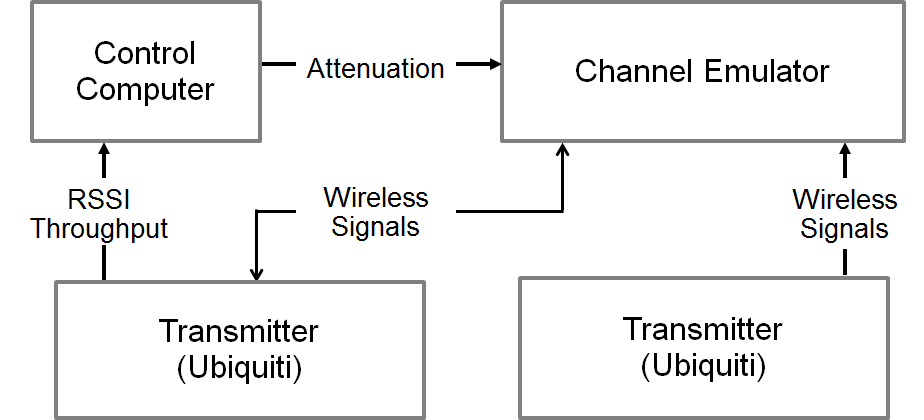
\includegraphics[width=85mm]{figure/emulator2}
\caption{Hardware Performance Experiment Setup}
\label{fig:in-door experiment}
\end{figure}

For this scenario, in a given band, we repeat the experiments under different configuration to get the throughput information across multiple bands in an ideal channel environment with different RSSI.
For each band, on the receiver side we capture the RSSI and report the throughput values from Iperf \cite{Iperf} each second. Based on these data,the performance database can be created.

Also, there is performance difference of each radio. However, our work does not focus on these issues. From the emulator experiment data, the throughput performance could be normalized for comparison. 
%the band adptation algorithm will extract the relationship between the contextual information and the target band.


%\subsection{Signal Level Context-aware information}
%There are two parts of this scenario in different environments, indoor and in-field. The experiments are done in the lab and on campus. We analyze the influence of the information amount for the prediction. 
\subsection{Experimental Design for In-field Data Collection}

To evaluate our algorithms, in-field experiments are taken for data collection.
The in-field experiments have 2 Gateworks nodes, two nodes are installed on two cars, one works as receiver, another works as transmitter moving in a public park as shown in \ref{fig:infield}.

\begin{figure}
\centering
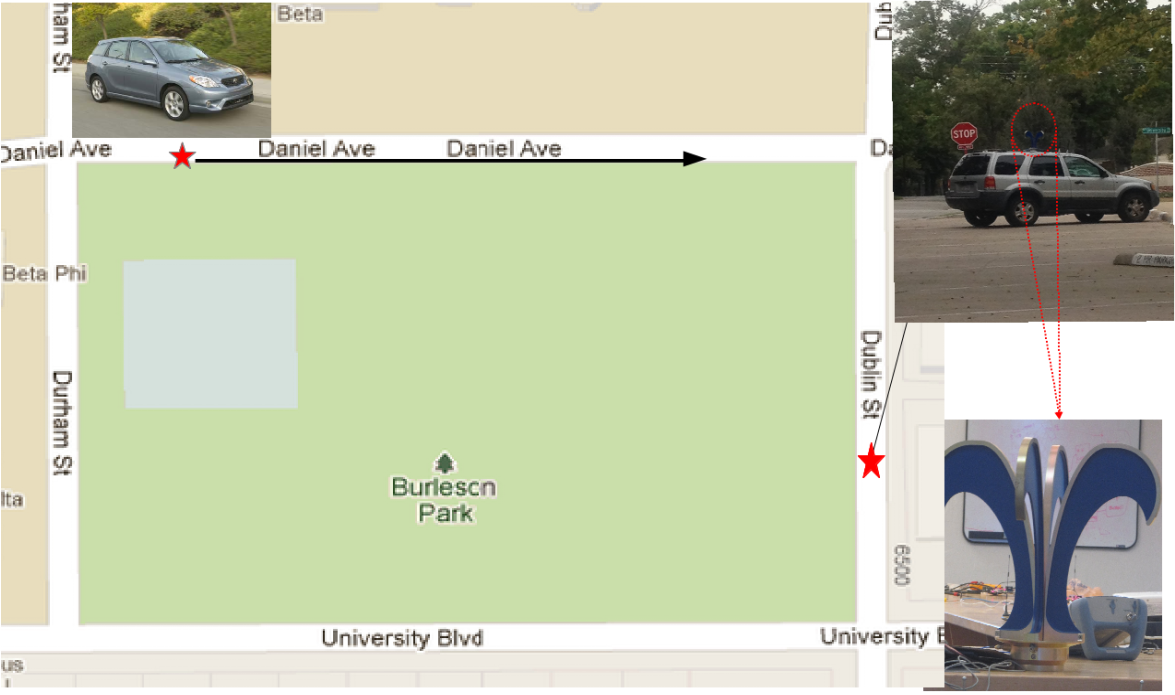
\includegraphics[width=85mm]{figure/infield}
\caption{In-field Experiment Setup}
\label{fig:infield}
\end{figure}


The same as in emulator experiments, we generate traffic and measure the throughput through Iperf. Then we dump all the transmitting packets and calculate the signal level from sniffer data in one receiver node. 
In receiver node, we dump all the packets it can received, then calculate the throughput and the signal level. We put the results in the algorithms to get the estimate optimize band, estimate throughput, measured throughput for evaluation.
One of the car park in a fixed location, then another car drive around the park for several loops to get the data with parameters. 

As shown in in \ref{fig:infield}, we use an multi-band antenna work with an spectrum analyzer to detect the signal in the air. All the activity can be seen on the data get from spectrum analyzer.
Also, all the 802.11 packets are dumped by Tcpdump installed on Gateworks wireless nodes \cite{jacobson1989tcpdump}. Then based on the time stamps, 802.11 packets can be recognized and only non 802.11 interference will be counted from the spectrum analyzer data.  
%Input spectrum analyzer process figure, explain

\begin{figure}
\centering
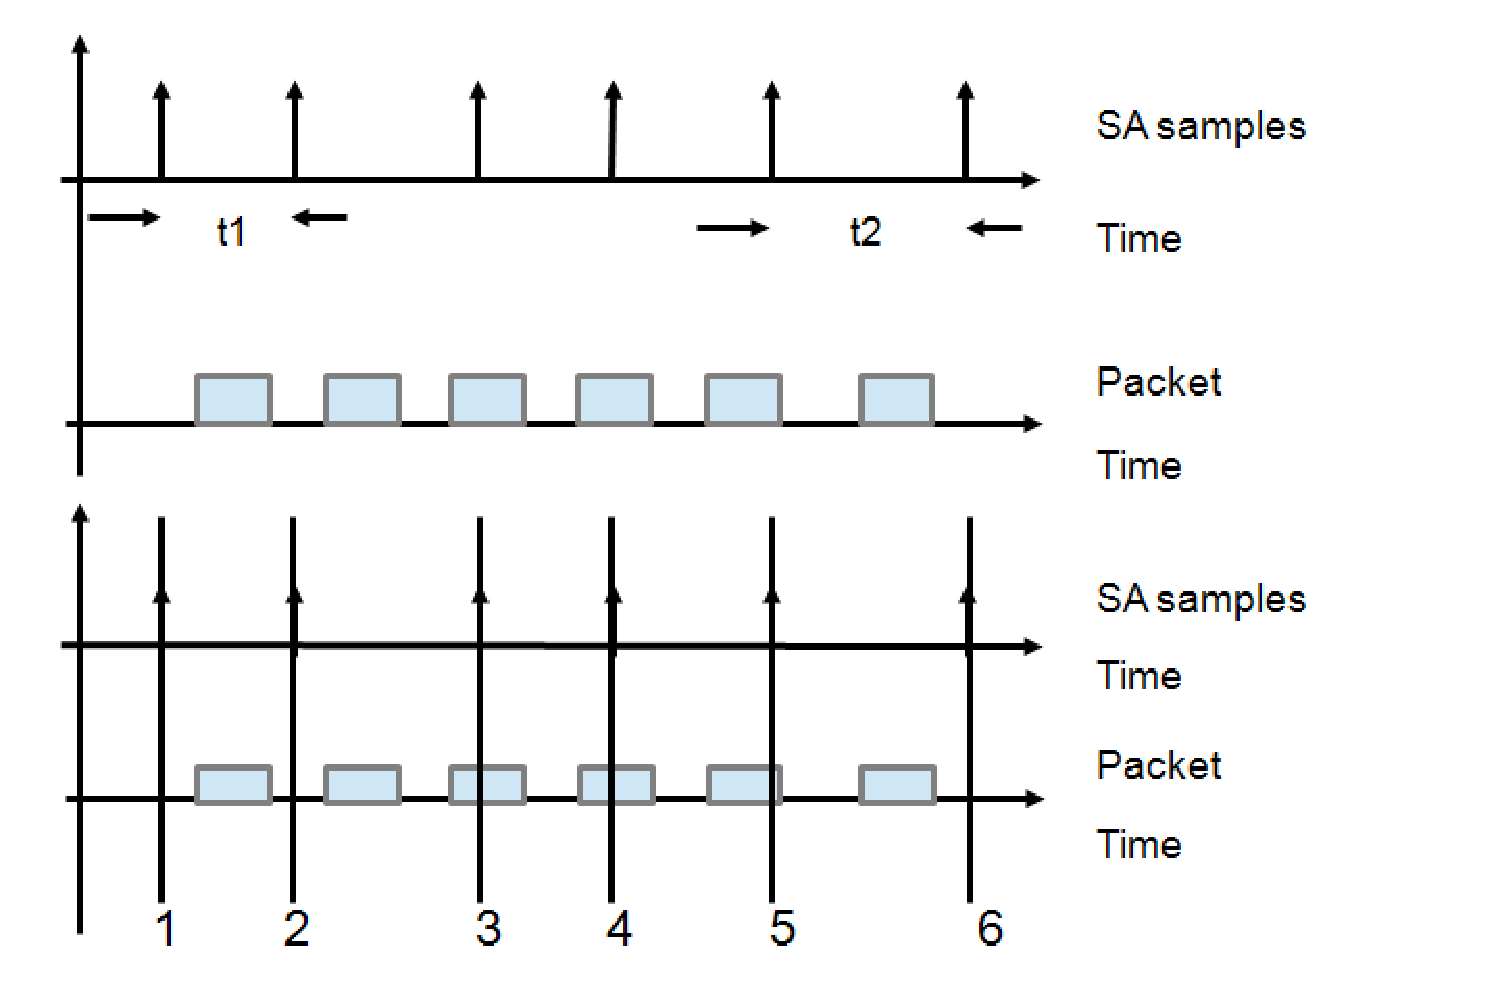
\includegraphics[width=85mm]{figure/sa_process}
\caption{Spectrum Analyzer Data Processing}
\label{fig:sa_process}
\end{figure}


The in-field data is processed offline. As discussed in \ref{subsec:ideal channel}, the throughput was normalized based on the emulator experiment to balance the diversity of hardware performance. Then, data from different devices and software is synchronized based on the GPS/System time stamps.

The in-field data will be divede into training data and testing data for \emph{Location Based Algorithm}, \emph{Machine Learning Algorithm} and \emph{Split Region Machine Learning Algorithm}.

%\subsubsection{Activity Level Measure} 
%Madwifi is the driver widely embedded in Linux based wireless operating system, as in OpenWRT \cite{Madwifi,Openwrt}. Madwifi provide an interface for sniffer to get the information of each packet.
%For the in-field scenario,
%to get the \emph{Activity Level,SNR} as the input of our algorithm, 
%we calculate from the dumped packets information. The transmitting rate and length of each packet can be captured by sniffer.%The \emph{Activity Level} is calculated by these information.

%to map the total received packets, our focused transmitter-receiver pair received packet, received signal power, background noise and interference. We use two Gateworks platform with Ubiquiti radios combining Agilent Spectrum Analyzer to collect data for our off-line analysis. We map these data synchronous through timestamp from GPS information on our testbed and the system time on the Spectrum Analyzer.

%To calculate the \emph{Activity Level}, the raw data we need is the total received packets and the focused transmitter-receiver pair received packets during a small time slot. 
%To measure the throughput and calculate the focused transmitter-receiver pair received packet(Focused RX packet) in a less than 1 second time slot, a socket program is generated for the experiments. The transmitter side could send packets in a 500ms duration, then turn off the transmission for another 500ms to meaure the interference. These raw data could be put into \ref{equation:Activity Level} calculate the activity level for the future prediction.


%in-field experiments design
%Gateworks, socket, spectrum analyzer
%\subsection{In-field Experiments}

%\subsubsection{Signal Measure}
%For the in-field experiments, the nodes has the same configuration. But we put the transmitter node and one receiver node in a location, the other receiver node on a car. In this scenario, the input of the frame work includes velocity, and all the context-aware database information and test information are collected from the receiver node on the car.

%We need the pure signal power from the transmitter to extract the ideal throughput from the context information we got from emulated channel experiments. It is impossible to get the interference during the transmitter sending period. So the transmitter is configured to turn on for a 500ms transmission to measure the throughput and the signal power(noise, interference and transmit power), and then turn off for another 500ms to measure the interference strength. 

%Fixme figure of the experiment flow

%SA utility
%The testbed could report the received strength, howerve, it could not update the value without transmission. The method we use to collect the signal strength is to record the spectrum activity through an Agilent Spectrum Analyzer. Agilent MXA N9020 Signal Analyzer could monitor a wide band spectrum and record the spectrum activity in a CSV file for a time point \cite{SA}. To get the continous record during the experiments, a MFC(Microsoft Foundation Class) dialog software is generated to control the spectrum analyzer to save the record file periodicly through Agilent I/O Command Expert\cite{MFC,AC}. We also record the signal strength on the testbed to match the record from spectrum analyzer.

%A node in a car works as the transmitter, and another node with the spectrum analyzer located in a fixed place work as the receiver. The car drive one loop on campus for a measurement of one band. During one loop, the throughput, RX packets, Focused RX packets, signal strength in transmission on and transmission off are collected. 

%Based on these collected data, the off-line data process are done with accuracy and improvement as metric to evaluate the methods.  
%

